
\chapter{Simulação em hardware}

Após a desenvolvimento da API descrita no capitulo anterior, pretendeu-se simular o sistema num contexto real. Para tal, planeou-se encontrar hardware que encaixasse no contexto deste projeto. Foram utilizados dois micro-controladores e alguns sensores. Neste capitulo será descrito cada um deles e o processo de desenvolvimento da respetiva simulação.  




\section{Micro-controladores}


Para o cenário anteriormente descrito foram utilizados dois micro-controladores bastante comuns no mercado: um Arduino Nano e um Raspberry Pi 3. Neste contexto, assume-se que o Arduino Nano é considerado um \ac{SM} que possui um conjunto de sensores enquanto que o Raspberry Pi 3 é um \ac{CM} que recebe os dados provenientes do \ac{SM} enviando-os para o servidor. 


\subsection{Arduino Nano}


O Arduino é fruto da evolução de um projeto italiano desenvolvido no ano de 2005, cujo o objetivo foi ser utilizado em projetos escolares de forma a ter um orçamento menor que outros sistemas de prototipagem disponíveis naquela época.

Tal como descrito no seu site oficial, um Arduino consiste numa plataforma \textit{open-source} de prototipagem eletrónica com \textit{hardware} e \textit{software} flexíveis e com elevada facilidade utilização[]. O Arduino é utilizado para projetos especialmente no contexto do \ac{IoT} e da robótica educativa.Neste micro-controlador, podem ser estendidos vários módulos, dependendo da tarefa que se quer que seja executada. 



O Arduino possui um conjunto de pinos que podem ser programados para funcionarem como entradas ou saídas fazendo com que o Arduino interaja com o meio externo para os mais diversos fins. Para além dos pinos de I/O exitem pinos de alimentação que Fornecem diversos valores de tensão que podem ser utilizados para transmitir energia elétrica aos diferentes componentes de um projeto. 

Na figura \ref{ard2} e \ref{ard1} apresenta-se uma imagem do arduino utilizado e a identificação dos diferentes pinos existentes, respectivamente. Na tabela \ref{caraarduino} encontram-se as principais características desta versão do Arduino. 


\begin{figure}[h]
	\centering
	\begin{minipage}[b]{0.5\textwidth}
		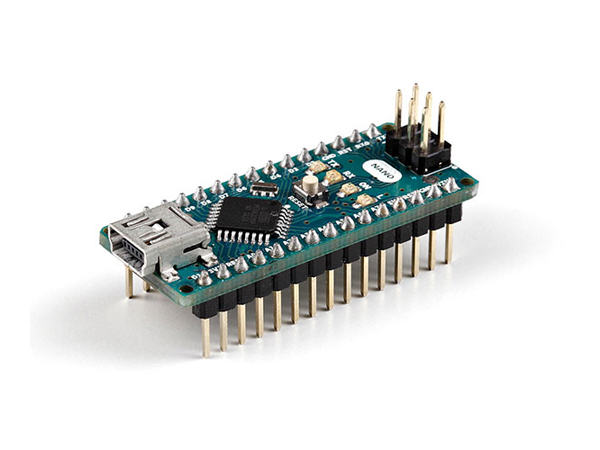
\includegraphics[width=\textwidth]{img/hardware/nano-img.jpg}
		\caption{Arduin Nano}
		\label{ard2}
	\end{minipage}
	\hfill
	\begin{minipage}[b]{0.3\textwidth}
		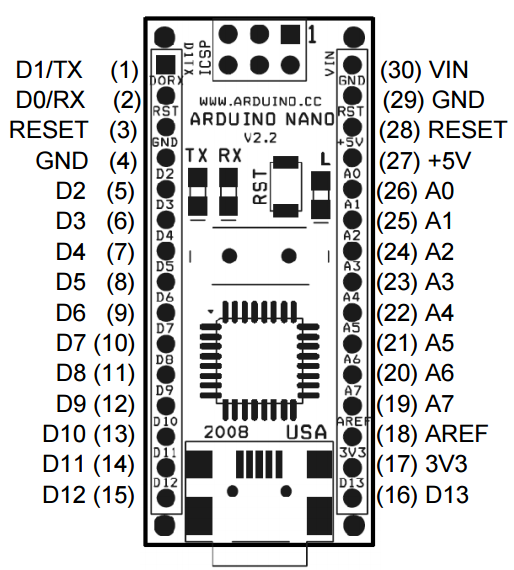
\includegraphics[width=\textwidth]{img/hardware/nano-esquema.png}
		\caption{Identificação dos pinos no Arduino Nano}
		\label{ard1}
	\end{minipage}
\end{figure}










\begin{table}[h]
	\centering
	
	\begin{tabular}{|
			>{\columncolor[HTML]{C0C0C0}}l |l|} \hline
		Microcontrolador & ATmega328 \\ \hline
		Tensão de operação & 5V \\ \hline
		Tensão de entrada & 7-12V \\ \hline
		Portas digitais & 14 (6 podem ser usadas como PWM) \\ \hline
		Portas analógicas & 8 \\ \hline
		Corrente nos pinos I/O & 40mA \\ \hline
		Memória Flash & 32KB (2KB usado no bootloader) \\ \hline
		Memória RAM (SRAM) & 2KB \\ \hline
		EEPROM & 1KB \\ \hline
		Velocidade do Clock & 16MHz \\ \hline
		Dimensões & 45 x 18mm \\ \hline
		LED Interno & Pino digital 13 \\ \hline
		Ligação USB & Ligação ao computador e alimentação \\ \hline
	\end{tabular}
	\caption{Características do sensor TTC 104}
	\label{caraarduino}
\end{table}







\newpage

\subsection{Raspberry Pi }

O Raspberry Pi (figura \ref{rasp1}) é considerado um micro-computador do tamanho de um cartão de crédito que possui um conjunto de \textit{hardware} integrado que tal como Arduino possibilita uma interação com o meio exterior. O principal objetivo deste poderoso componente consistiu em promover o ensino da ciência da computação em escolas de ensino básico. 
O Raspberry Pi foi desenvolvido no Reino Unido pela \textit{Raspberry Pi Foundation}.




\begin{figure}[h]
	\centering
	\begin{minipage}[b]{0.4\textwidth}
		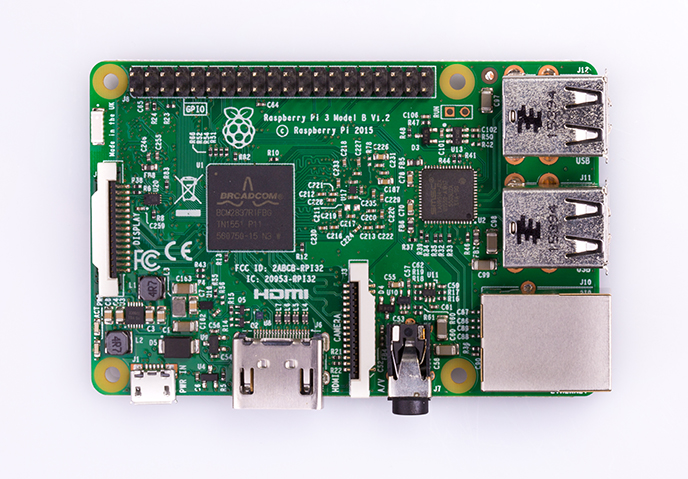
\includegraphics[width=\textwidth]{img/hardware/rasp3-img.jpg}
		\caption{Raspberry Pi 3}
		\label{rasp1}
	\end{minipage}
	\hfill
	\begin{minipage}[b]{0.5\textwidth}
		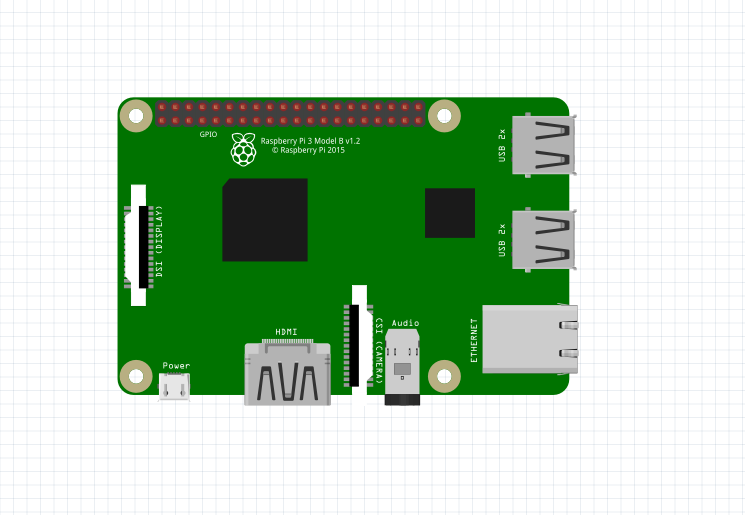
\includegraphics[width=\textwidth]{img/hardware/rasp-esquema.PNG}
		\caption{Identificação dos principais componentes no Raspberry Pi 3 }
	\end{minipage}
\end{figure}




\begin{table}[h]
	\centering

	\begin{tabular}{|
			>{\columncolor[HTML]{C0C0C0}}l |l|l|}
		\hline
		& \cellcolor[HTML]{C0C0C0}\textbf{Raspberry Pi 3 Model B} & \cellcolor[HTML]{C0C0C0}\textbf{Raspberry Pi 2 Model B 1.2} \\ \hline
		\textbf{Processor Chipset} & \begin{tabular}[c]{@{}l@{}}Broadcom BCM2837\\ 64Bit  Quad Core \\ Processor powered \\ Single Board Computer\\ running at 1.2GHz\end{tabular} & \begin{tabular}[c]{@{}l@{}}Broadcom BCM2837 64Bit \\ Quad Core Processor \\ powered Single Board \\ Computer running at \\ 900MHz\end{tabular} \\ \hline
		\textbf{Processor Speed} & QUAD Core @1.2 GHz & QUAD Core @900 MHz \\ \hline
		\textbf{RAM} & 1GB SDRAM @ 400 MHz & 1GB SDRAM @ 400 MHz \\ \hline
		\textbf{Storage} & MicroSD & MicroSD \\ \hline
		\textbf{USB 2.0} & 4x USB Ports & 4x USB Ports \\ \hline
		\textbf{\begin{tabular}[c]{@{}l@{}}Max Power \\ Draw/voltage\end{tabular}} & 2.5A @ 5V & 1.8A @ 5V \\ \hline
		\textbf{GPIO} & 40 pin & 40 pin \\ \hline
		\textbf{Ethernet Port} & Yes & Yes \\ \hline
		\textbf{WiFi} & Built  in (802.11n) & No \\ \hline
		\textbf{Bluetooth LE} & Built in (4.1) & No \\ \hline
	\end{tabular}
	\caption{Comparação entre versão 2 e 3 do Raspberry Pi}
	\label{my-label}
\end{table}







\newpage
\section{Sensores}

Nesta secção serão apresentados os sensores utilizados na simulação e as suas principais características. Todos os sensores foram escolhidos tendo em conta o seu enquadramento no projeto e a sua disponibilidade no laboratório. Todos os sensores que se apresentam encontram-se ligados a um Arduino nano. 


\subsection{Temperatura}

Como sensor de temperatura foi utilizado um termístor do tipo \ac{NTC}. Como vimo anteriormente, um termístor é um semicondutor sensível à temperatura i.e. cujo o coeficiente de variação da resistência com a temperatura é negativa, ou seja, quando a temperatura sobe então consequentemente a resistência diminui. 

Na figura \ref{esquema-temp} encontra-se o esquema de ligação deste componente e na tabela \ref{table-temp} as propriedades principais. 

\begin{figure}[h]
	\centering
	\begin{minipage}[b]{0.4\textwidth}
		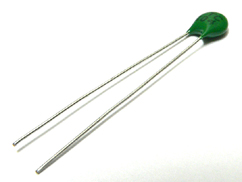
\includegraphics[width=\textwidth]{img/hardware/temperatura.jpg}
		\caption{TTC 104 NTC}
	\end{minipage}
	\hfill
	\begin{minipage}[b]{0.4\textwidth}
		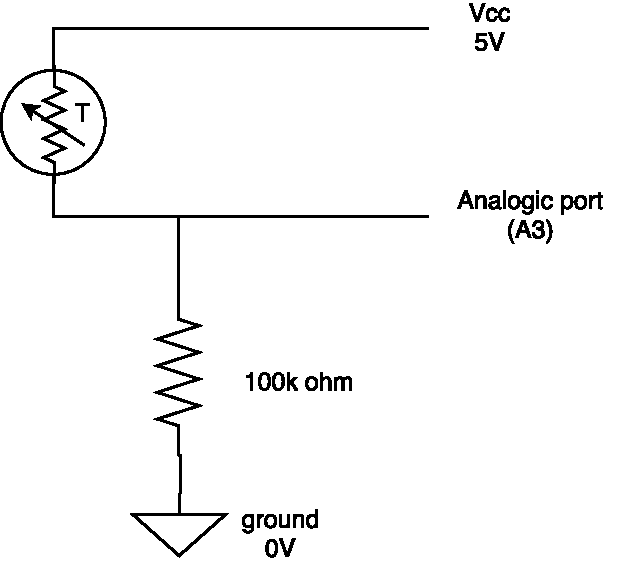
\includegraphics[width=\textwidth]{img/hardware/temp-esquema.pdf}
		\caption{Esquema eletrotécnico da ligação do sensor de temperatura}
		\label{esquema-temp}
	\end{minipage}
\end{figure}



\begin{table}[h]
	\centering
	
	\begin{tabular}{|
			>{\columncolor[HTML]{C0C0C0}}l |l|} \hline
		Dimensão & 5mm \\ \hline
		Resistência & 100K $\Omega$  \\ \hline
		Valor máximo & +125C \\ \hline
		Valor mínimo & -30C \\ \hline
		Nível de confiança & + - 10\% \\ \hline
		Preço & 0.35 \euro/unidade \\ \hline
	\end{tabular}
	\caption{Características do sensor TTC 104 \cite{temp-dta}}
	\label{table-temp}
\end{table}



\subsection{Luminosidade}

Para simular a luminosidade incidente foi utilizado um sensor do tipo foto-resistência. Este sensor, também conhecido como \ac{LDR}, não é mais do que uma resistência variável cujo o seu valor varia conforme a intensidade da luz que incide sobre ele i.e. à medida que a intensidade da luz aumenta, a sua resistência diminui. Este sensor tem múltiplas aplicações, entre as quais se destaca a monitorização solar, indicador da posição do sol (up/down), alarmes anti-roubo, alarme para abertura/fecho de portas entre outras. 

Como vimos na secção X do capitulo do Estado de Arte é um sensor de baixo custo e bastante fácil de utilização. Na figura \ref{lum-esquema} encontra-se o esquema de ligação do componente e na tabela \ref{lum-cara} são apresentadas as principais características do sensor utilizado. 







\begin{figure}[h]
	\centering
	\begin{minipage}[b]{0.4\textwidth}
		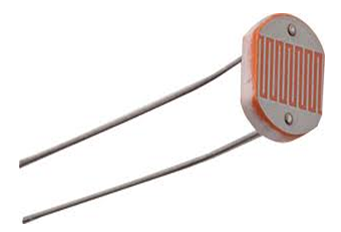
\includegraphics[width=\textwidth]{img/hardware/luminosidade.png}
		\caption{Sensor foto-resistência GL5528}
	\end{minipage}
	\hfill
	\begin{minipage}[b]{0.4\textwidth}
		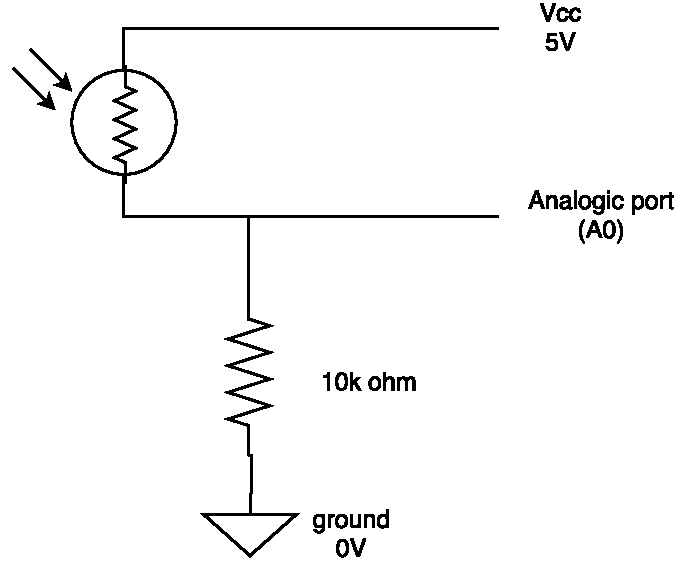
\includegraphics[width=\textwidth]{img/hardware/lumi_esquema.pdf}
		\caption{Esquema eletrotécnico da ligação do sensor de luminosidade}
		\label{lum-esquema}
	\end{minipage}
\end{figure}











\begin{table}[h]
	\centering
	
	\begin{tabular}{|
			>{\columncolor[HTML]{C0C0C0}}l |l|} \hline
		Diâmetro & 5mm \\ \hline
		Tensão máxima & 150VDC \\ \hline
		Potência máxima & 100mW \\ \hline
		Tensão de operação & -30 C a 70 C \\ \hline
		Espectro &540nm \\ \hline
		Comprimento com terminais & 32mm \\ \hline
		Resistência no escuro &1 M (Lux 0) \\ \hline
		Resistência na luz &10-20 Komega (Lux 10) \\ \hline
		Material & Carbono \\ \hline
		Preço & 0.22 \euro/unidade \\ \hline
	\end{tabular}
	\caption{Características do sensor GL5528 \cite{lum-data}}
	\label{lum-cara}
\end{table}


\subsection{Sensor de nível líquido}

Este sensor não é mais do que um interruptor que é ativo sempre que um determinado líquido ultrapassa o mesmo. Sempre que algum líquido atingir o pedaço de plástico este irá subir ativando assim o circuito. 
Na figura \ref{esquem-liquido} encontra-se o esquema da ligação deste sensor.




\begin{figure}[h]
	\centering
	\begin{minipage}[b]{0.4\textwidth}
		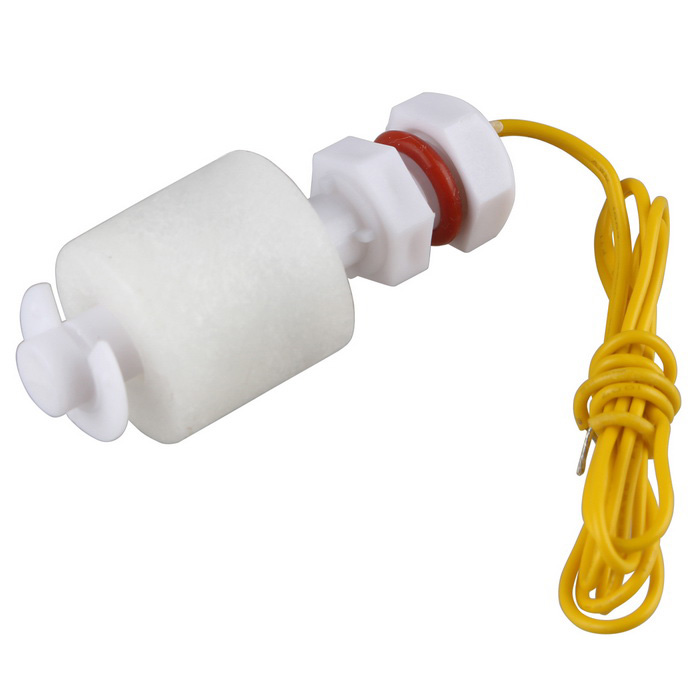
\includegraphics[width=\textwidth]{img/hardware/liquido.JPG}
		\caption{\textit{Water Level Switch Liquid Level Sensor Plastic Ball Float}}
	\end{minipage}
	\hfill
	\begin{minipage}[b]{0.4\textwidth}
		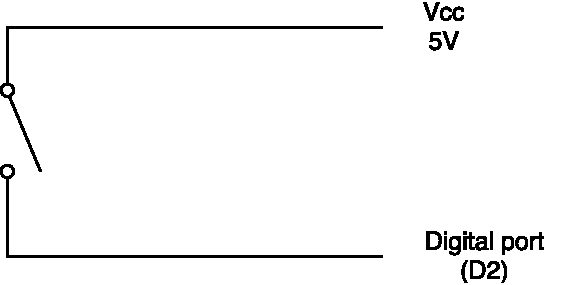
\includegraphics[width=\textwidth]{img/hardware/sw_esquema.pdf}
		\caption{Esquema eletrotécnico da ligação do sensor de nível líquido}
		\label{esquem-liquido}
	\end{minipage}
\end{figure}




\subsection{Simulador de válvula para transferências de águas}

Para a simulação de uma válvula que permitirá as transferência de água doce e salgada foi utilizado um simples \textit{led}. Este possibilita facilmente identificar através da ativação do \textit{led} se a válvula se encontra ativa ou não. 


\begin{figure}[h]
	\centering
	\begin{minipage}[b]{0.4\textwidth}
		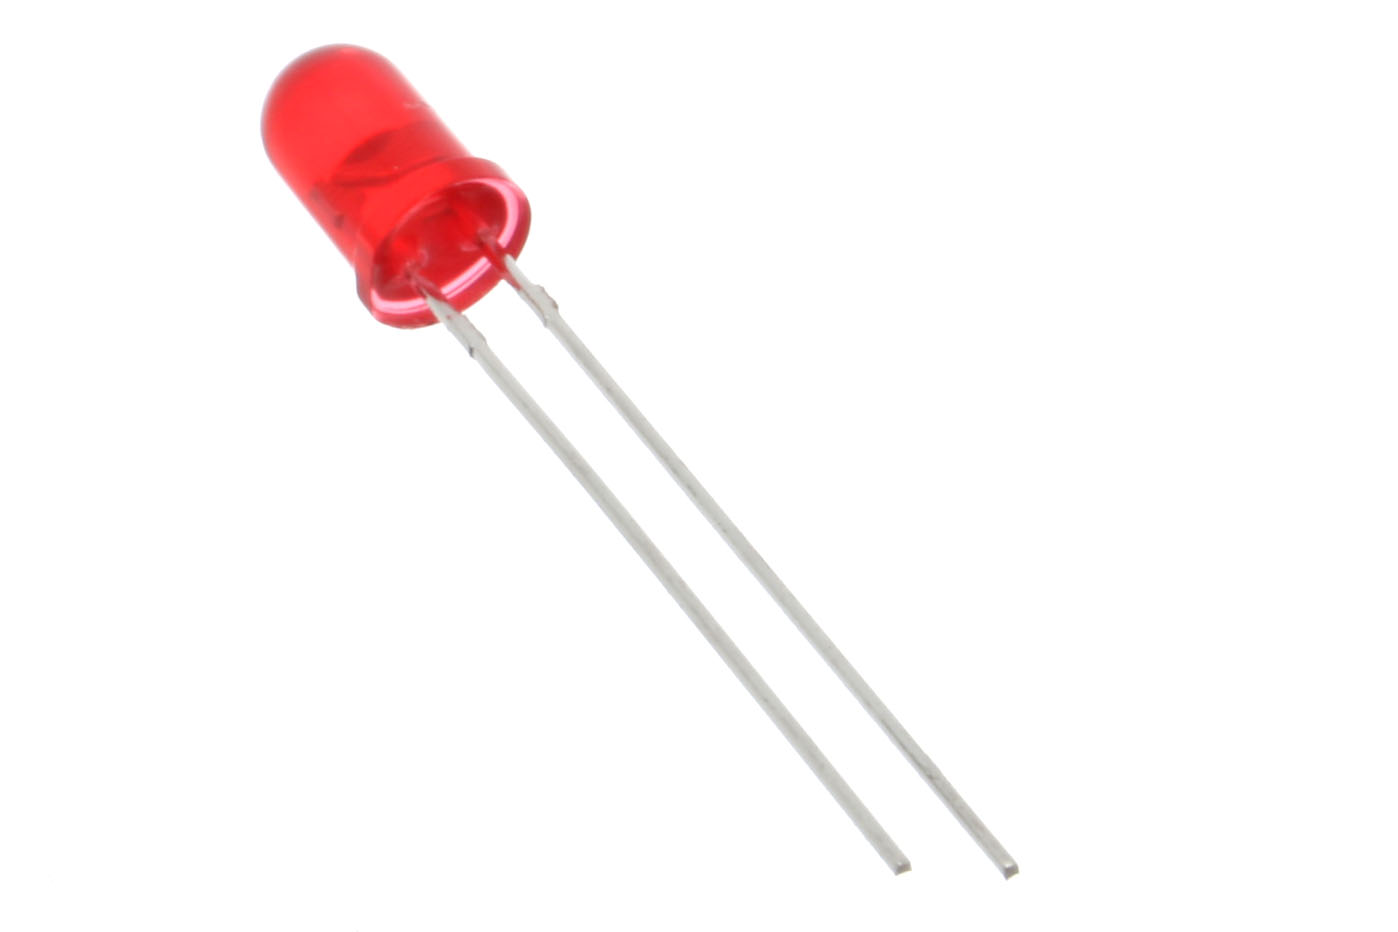
\includegraphics[width=\textwidth]{img/hardware/led.jpg}
		\caption{Led simples.}
	\end{minipage}
	\hfill
	\begin{minipage}[b]{0.4\textwidth}
		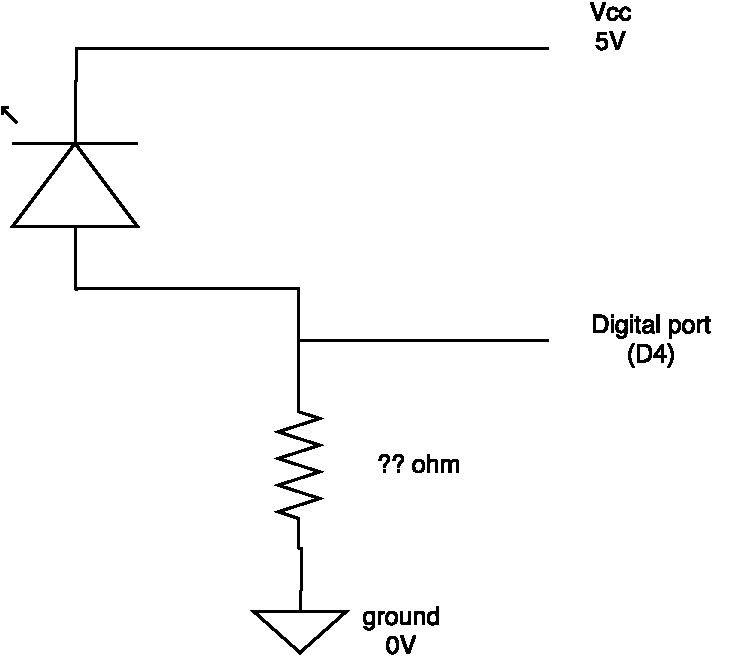
\includegraphics[width=\textwidth]{img/hardware/led_esquema.pdf}
		\caption{Esquema eletrotécnico da ligação do led}
	\end{minipage}
\end{figure}




\newpage
\section{Comunicação}

Nesta secção, será apresentado o tipo de comunicação para este cenário de simulação. Pretendeu-se que cada um dos módulo ficassem isolados entre si, o que implicou o estudo e respetiva escolha de algumas tecnologias de comunicações sem fio. Neste caso, foram escolhidas as seguintes: 

\begin{itemize}
	\item \textbf{Bluetooth}: utilizado para a comunicação entre o Arduino (\ac{SM}) e o Raspberry Pi 3 (\ac{CM}). No Arduino foi utilizado um módulo Bluetooth HC-06 e no Raspberry Pi 3 foi utilizado o seu próprio módulo interno. 
	\item \textbf{Wifi}: utilizado para a comunicação entre o Raspberry Pi 3 (\ac{CM}) e o servidor. 
\end{itemize}


O esquema da figura \ref{esquemcomm} pretende esquematizar os tipos de comunicação envolvidos nesta simulação para cada um dos componentes. 

\begin{figure}[!htb]
	\centering
	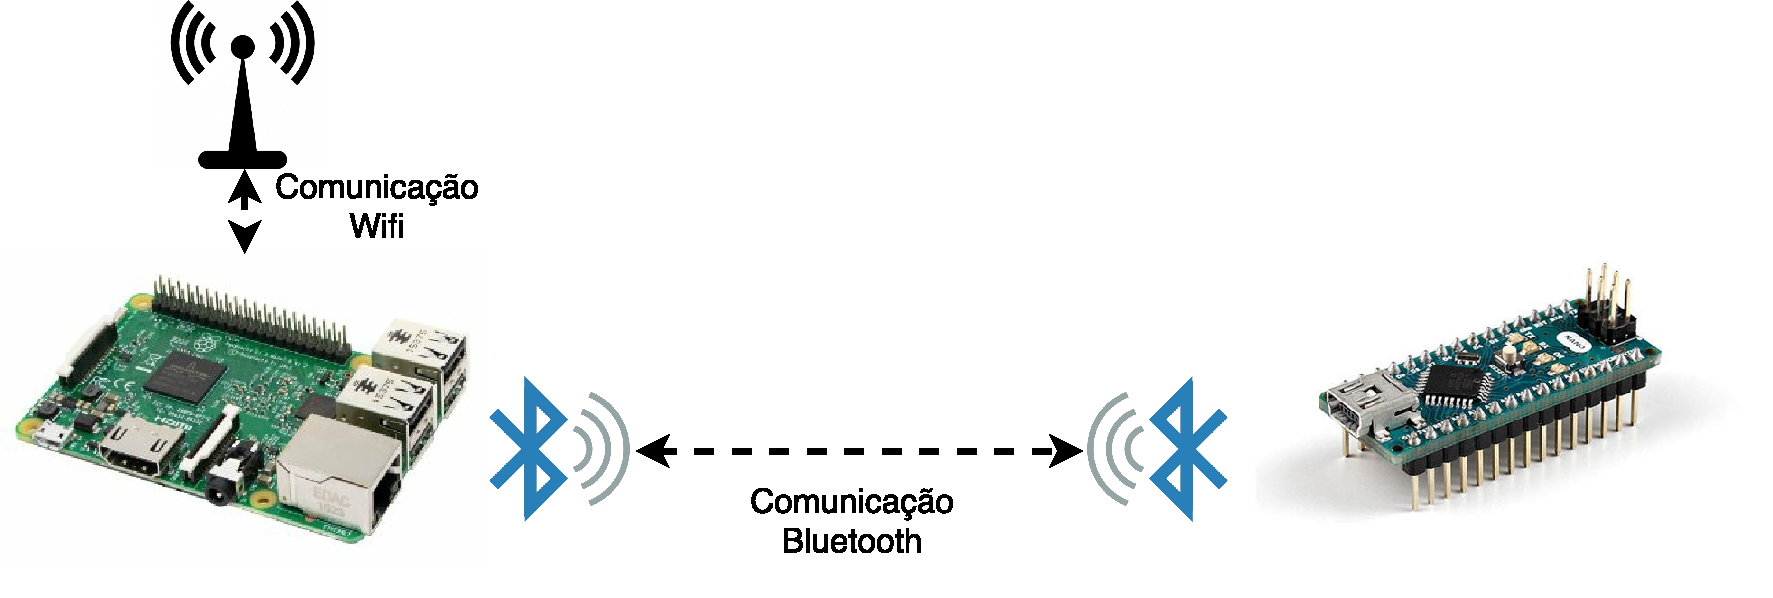
\includegraphics[width=\linewidth]{img/comm-blue/HW-geral.pdf}
	\caption{Arquitetura lógica}
	\label{esquemcomm}
\end{figure}




\subsection{Módulo bluetooth HC-06}



Este módulo bluetooth HC-05 oferece uma forma fácil e barata de comunicação com seu projeto Arduino. Diferente do modelo HC-06, suporta tanto o modo mestre como escravo, além de ter uma fácil configuração.

Em sua placa existe um regulador de tensão e você poderá alimentar com 3.3 a 5v, bem como um LED que indica se o módulo está pareado com outro dispositivo. Possui alcance de até 10m.

 é mais uma forma simples e barata de enviar e receber informações remotamente.
 

\newpage
\begin{figure}[h]
	\centering
	\begin{minipage}[b]{0.4\textwidth}
		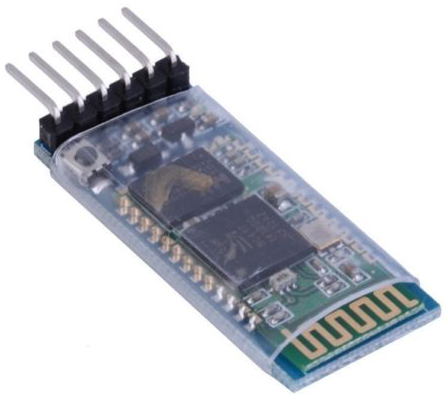
\includegraphics[width=\textwidth]{img/hardware/bluetooth_zs-040.png}
		\caption{Flower one.}
	\end{minipage}
	\hfill
	\begin{minipage}[b]{0.4\textwidth}
		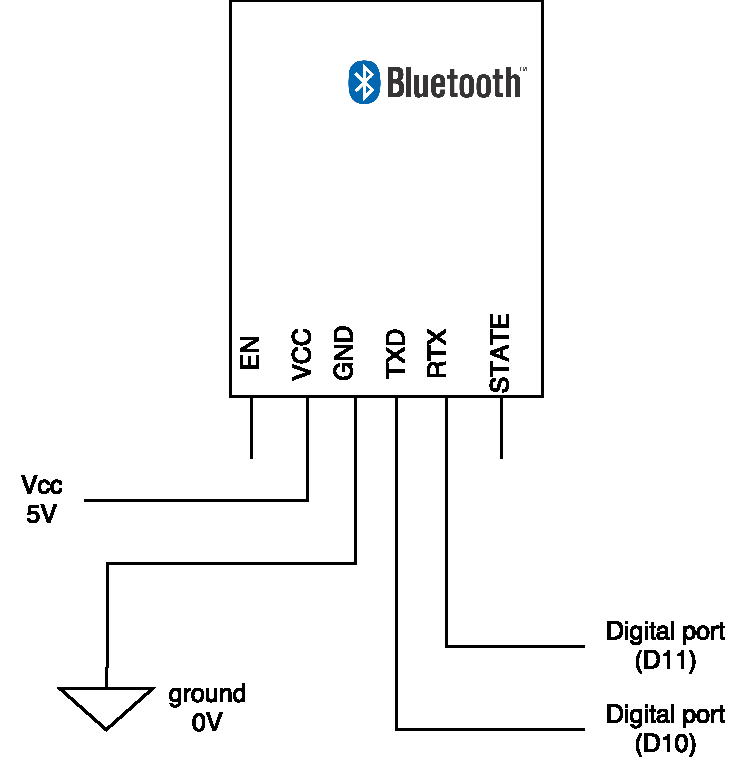
\includegraphics[width=\textwidth]{img/comm-blue/electronic-sensors.pdf}
		\caption{Esquema eletrotécnico da ligação do módulo bluetooth}
	\end{minipage}
\end{figure}



\begin{table}[h]
	\centering
	
	\begin{tabular}{|
			>{\columncolor[HTML]{C0C0C0}}l |l|} \hline
		Diâmetro & 5mm \\ \hline

		Protocolo Bluetooth& v2.0+EDR \\ \hline 
		Frequência& 2,4GHz Banda ISM \\ \hline
		Segurança& Autentificação e Encriptação \\ \hline
		Tensão& 3,3v (2,7-4.2v) \\ \hline
		Alcance& 10m \\ \hline
		Dimensões& 26,9 x 13 x 2,2mm \\ \hline
		Peso& 9,6g \\ \hline
		Preço&32\euro /unidade  \\ \hline
	\end{tabular}
	\caption{Características do sensor GL5528 \cite{lum-data}}
	\label{lum-cara}
\end{table}



%http://www.instructables.com/id/Modifying-the-AT-Codes-on-a-HC-05-With-the-Code-ZS/


%http://www.arduinoecia.com.br/2013/03/modulo-bluetooth-jy-mcu-configuracao.html






\newpage
\section{Implementação}

Nesta secção pretende-se explicar a implementação a nível de \textit{software} no contexto desta simulação para cada um dos micro-controladores. 


\subsection{Arduino}

No que diz respeito ao Arduino Nano (\ac{SM}), numa fase inicial,  procedeu-se à ligação dos diversos componentes anteriormente apresentados na \textit{breadboard} tal como se encontra apresentado no Anexo \ref{interlapd}. Para auxiliar o desenvolvimento de \textit{software} foi utilizada a versão 1.8.1 do \ac{IDE} do próprio Arduino\footnote{https://www.arduino.cc/en/Main/Software}.  

Seguidamente apresenta-se a implementação necessária a nível de sensores e de comunicação. 

\subsubsection{Sensores}

Foram desenvolvidos os seguintes métodos que permitem aceder aos valores lidos de cada um dos sensores. Para além disso, foi criado um método que permite alterar o estado do válvula para transferência de água. 

\begin{itemize}
	\item \texttt{int readTemperature(int port)}: é efetuada uma leitura no porto analógico. Após a leitura este é convertido para ºC (graus Celsius)
	
	\item \texttt{long readLuminosity(int port)}: 
	
	\item \texttt{int readWaterValve(int port)}: é efetuada uma leitura no porto digital através do método \texttt{digitalRead}. 
	
	\item \texttt{int readWaterLevel(int port)}: é efetuada uma leitura no porto digital através do método \texttt{digitalRead}.
	
	 
	\item \texttt{void setWaterValve(int port, int state)}: se a variável \texttt{state} for 1 então o porto é colocado a \texttt{HIGH} (1) através do método \texttt{digitalWrite}, caso contrário é colocado a \texttt{LOW} (0)
	
\end{itemize}

Inicialmente procedeu-se à leitura de cada sensor de forma individual de modo a garantir o seu total funcionamento. Sempre que é feita um pedido de leitura dos sensores pelo \ac{CM} os valores são enviados com o seguinte formato: 

\begin{equation} 
\label{eq:someequation}
\texttt{<temperatura>;<nível\_água>;<luminosidade>;<estado\_válvula>}
\end{equation}

\subsubsection{Comunicação}


Numa primeira fase procedeu-se à comunicação entre o \ac{SM} e \ac{CM} através de porta série. Seguidamente resolveu-se incorporar o módulo bluetooth de modo a tornar cada módulo independente. De módulo de interagir com o módulo bluetooth utilizou-se o package \texttt{SoftwareSerial.h} disponível no Arduino. Decidiu-se que caso o módulo bluetooth recebesse valores de 0 a 2 tinha diferentes comportamentos: 

\begin{itemize}
	\item \textbf{0}: ativação (ligar) da válvula; 
	\item \textbf{1}: desativação (desligar) da válvula; 
	\item \textbf{2}: recebe dados obtidos pelos sensores no formato definido em (\ref{eq:someequation})
\end{itemize}

Antes de proceder à implementação de envio e receção de dados por bluetooth no Raspberry Pi 3 optou-se por testar este mecanismo através de uma aplicação Android existente na \textit{Play Store} chamada de \textit{Bluetooth Terminal HC-05}\footnote{https://play.google.com/store/apps/details?id=project.bluetoothterminal}

\subsection{Raspberry Pi}


\subsubsection{Comunicação}


Como é possível observar na figura \ref{esquemcomm}, para a comunicação no Raspberry Pi (\ac{CM}) entre o Arduino (\ac{SM}) foi utilizado o modulo interno de bluetooth 4.1 que este incorpora no seu hardware. Para tal, foi desenvolvido um \textit{script} em Python que permite o seguinte: 


\begin{enumerate}
	\item a dese com 
\end{enumerate}

Para permitir o acesso aos recursos do sistema Bluetooth foi utilizada uma extensão (\textit{package}) do Python denominado de \textit{pybluez}\footnote{https://github.com/karulis/pybluez}. 
 

 

\section{Considerações finais}


>1 fase testar coneccao arduino to rasp via porta serie; foi criado um script em python para processar info e enviar para o servidor através da API 

>2 fase : necessidade de tornar um módulo isolado sem necessidade de fio; foi testado um modulo wifi e bluetooth; 

>neste contexto modulo wifi nao!... pretende-se que os sensor moduels sejam de baixo custo e low power. foi utilizado um modulo bluetooth; foi testada a conexao da comm bluetooth através de uma client disponveil na google play bluetooth terminal HC-05 


> 
pq nao foi usado um sensor de salinidade? nao havia orçamento.. 



 

